% SPDX-License-Identifier: LPPL-1.3c
% Copyright (C) 2026 Christophe Jorssen
% Author and Current Maintainer: Christophe Jorssen <christophe.jorssen@gmail.com>
% LPPL maintenance status: maintained
% This file is part of luafemm. See LICENSE and LICENSES.md for its terms.
\section{Image charges and material response}
\label{sec:electric-images}
\index{electrostatics!image charges}
\index{electrostatics!induced charge}

Superposition is exact for prescribed charges in a homogeneous linear medium.
A conductor or dielectric interface generally changes the solution: drawing
a metal rectangle over an analytical field does not make the field satisfy
the conductor's boundary condition. Some geometries admit an exact image
construction. It can be used immediately with the analytical point-charge
nodes, provided that the physical region and the fictitious sources are
identified explicitly.

\subsection{A charge above a grounded infinite plane}
Place a charge $q$ at $(0,a)$, with $a>0$, above the grounded plane $y=0$.
In the physical half-space $y>0$, the potential is
\[
 V(x,y)=\frac{q}{4\pi\epsilon}
 \left[\frac{1}{\sqrt{x^2+(y-a)^2}}
       -\frac{1}{\sqrt{x^2+(y+a)^2}}\right].
\]
An image charge $-q$ at $(0,-a)$ makes $V(x,0)=0$ everywhere on the plane.
This is a three-dimensional solution viewed in a plane through the real
charge and the surface normal. It is not the logarithmic potential of an
infinite charged wire. The conductor occupies $y\leq0$; the image is a
mathematical device, not a second physical charge inside the metal.

\luafemmexamplebegin{electric-images}
\Needspace{22\baselineskip}
\begin{codeexample}[width=0pt]
\begin{tikzpicture}[femm/electrostatic={
    xmin=-2.5,xmax=2.5,ymin=0,ymax=2.6},scale=1.1]
  \fill[gray!18] (-2.5,-.18) rectangle (2.5,0);
  \draw[thick] (-2.5,0)--(2.5,0);
  \node[below] at (0,-.18) {$V=0$};
  \node[femm/point charge={charge=1e-12,exclusion radius=.13},
    fill=red!15] at (0,1) {$+$};
  \node[overlay,opacity=0,
    femm/point charge={charge=-1e-12}] at (0,-1) {};
  \pic[femm/electric={lines per charge=14}] {femm electric field};
  \pic[femm/electric={levels={.1,.3,.6,1,2}}] {femm equipotentials};
  \path[femm/electric profile={name=plane field,samples=101}]
    (-2.5,0)--(2.5,0);
\end{tikzpicture}
\end{codeexample}

The default length unit is centimetres, so $a=1\,\mathrm{cm}$ here;
$q=1\,\mathrm{pC}$. The invisible node uses ordinary TikZ |overlay| and
|opacity| options: it remains a source but does not enlarge the picture's
bounding box. The analytical view window clips the result to $y\geq0$.
It neither removes the image from the calculation nor imposes a numerical
boundary. The grey strip and its label are ordinary drawing commands.

The surface normal from the metal into the dielectric is $+\mathbf e_y$.
Consequently the induced free surface charge density is
\[
 \sigma(x)=D_y(x,0^+)=-\frac{qa}{2\pi(x^2+a^2)^{3/2}}.
\]
The profile captures the same model used for the field lines. Its $D_y$
component is in $\mathrm{C/m^2}$; a native PGFPlots filter changes only the
display unit to $\mathrm{nC/m^2}$. The independent image formula provides a
useful check on signs, coordinates and unit conversion.

\Needspace{20\baselineskip}
\begin{codeexample}[width=0pt]
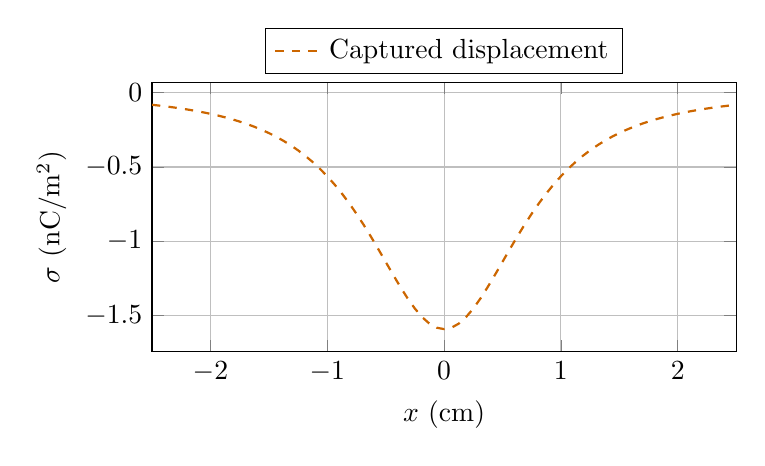
\begin{tikzpicture}
  \begin{axis}[width=9cm,height=5cm,xmin=-2.5,xmax=2.5,
    xlabel={$x$ (cm)},ylabel={$\sigma$ ($\mathrm{nC/m^2}$)},
    grid=major,legend style={at={(.5,1.03)},anchor=south}]
    \femmelectricplot[profile=plane field,component=Dy,abscissa=x,
      plot options={blue,thick,mark=none,
        y filter/.expression={1e9*y}}]
    \addlegendentry{Captured displacement}
    \addplot[orange!80!black,dashed,thick,domain=-2.5:2.5,
      samples=81] {-5/pi/(1+x*x)^1.5};
    \addlegendentry{Image formula}
  \end{axis}
\end{tikzpicture}
\end{codeexample}
\luafemmexampleend{electric-images}

This curve is a section of a surface density, not a line-charge density.
Integrating it over $x$ alone does not give the conductor's total charge.
With cylindrical radius $r$ on the plane, the correct integral is
$\int_0^\infty\sigma(r)\,2\pi r\,\mathrm dr=-q$.
Image constructions for curved or finite conductors need their own solution;
reusing this pair of nodes does not approximate an arbitrary electrode.

\subsection{What a dielectric correction must satisfy}
\label{sec:electric-correction}
At a dielectric interface without prescribed free surface charge, the
potential and tangential $\mathbf E$ are continuous, and the normal
$\mathbf D$ is continuous. Simply evaluating the same Coulomb field with
one permittivity on either side violates these conditions.

For example, a point charge in medium $\epsilon_1$ above a plane adjoining
medium $\epsilon_2$ has the reflected image strength
\[
 q'=\frac{\epsilon_1-\epsilon_2}{\epsilon_1+\epsilon_2}\,q.
\]
In medium 1, use the real source and its reflected image, both with
permittivity $\epsilon_1$. In medium 2, the potential can instead be written
as that of $q''=2\epsilon_2q/(\epsilon_1+\epsilon_2)$ at the real source's
position, evaluated with permittivity $\epsilon_2$. These are two regional
expressions of one solution; neither expression alone applies everywhere.

More generally, write $V=V_s+u$, where $V_s$ is a known source solution in a
homogeneous reference medium $\epsilon_b$. The correction $u$ satisfies
\[
 \int_\Omega \boldsymbol\epsilon\nabla u\mathbin\cdot\nabla w\,\mathrm d\Omega
 =-\int_\Omega(\boldsymbol\epsilon-\epsilon_b I)
        \nabla V_s\mathbin\cdot\nabla w\,\mathrm d\Omega
\]
for test functions $w$ vanishing on prescribed-potential boundaries, with
$u=g-V_s$ wherever the total potential is prescribed as $g$. This displayed
form assumes that all prescribed sources are included in $V_s$ and that the
remaining boundary is a regular axis or has prescribed potential. Other
boundary conditions require their own source-field terms. Taking
$\boldsymbol\epsilon=\epsilon_b I$ in a neighbourhood of every singularity
keeps the contrast integral regular. The guard neighbourhood is not a
softening radius: the physical singularity remains.

In planar geometry, an isolated source in the section represents an infinite
line, with strength $\lambda$ in C/m and
$V_s=-\lambda\log(d/d_0)/(2\pi\epsilon_b)$. In axisymmetry, a point charge on
the symmetry axis has strength $q$ in C and
$V_s=q/(4\pi\epsilon_b d)$; volume and surface integrals include the full
$2\pi r$ measure. An off-axis isolated point has no axial symmetry.
Neither construction permits arbitrary coplanar three-dimensional charges
to be corrected by a two-dimensional planar finite-element solve.

These equations explain why analytical superposition and the finite-element
models have distinct physical source interfaces. The public
|model=source correction| provider implements this formulation with tensor contrasts and
additional boundary terms; see Section~\ref{sec:electric-hybrid}. Its dedicated nodes
distinguish planar line strengths from axial point charges. In particular,
|femm/point charge| remains an analytical Coulomb source and cannot be added
to either numerical provider. Exact image constructions remain useful
independent solutions where their assumptions apply.

The distinction also matters in postprocessing. A potential consisting of an
analytical kernel plus a piecewise affine correction does not have a constant
gradient within a triangle. Raw finite-element line tracing and linear
equipotential interpolation cannot be reused unchanged. Ideal singular
sources have divergent total self-energy; excluding them from a drawing
does not define a finite energy or a force prescription. The explicitly
subtracted interaction energy and total Maxwell contour of
Section~\ref{sec:electric-source-energy} supply separate finite observables. Native FEMM answer
files contain nodal potentials, so they cannot preserve an unevaluated
analytical kernel and its exact off-node field.
